\documentclass[12pt]{article}

\addtolength{\textwidth}{1.3in}
\addtolength{\oddsidemargin}{-.65in} %left margin
\addtolength{\evensidemargin}{-.65in}
\setlength{\textheight}{9in}
\setlength{\topmargin}{-.5in}
\setlength{\headheight}{0.0in}
\setlength{\footskip}{.375in}
\renewcommand{\baselinestretch}{1.0}
\renewcommand{\thesection}{\Roman{section}} 
\renewcommand{\thesubsection}{\thesection.\Roman{subsection}}
\linespread{1.5}

\usepackage[pdftex,
bookmarks=true,
bookmarksnumbered=false,
pdfview=fitH,
bookmarksopen=true]{hyperref}
\usepackage[pdftex]{graphicx}
%\usepackage{pdfpages}

\usepackage[usenames,dvipsnames,svgnames,table]{xcolor}
\usepackage{cite}
\usepackage{times, verbatim,bm,pifont,pdfsync}
%\usepackage[hang,flushmargin]{footmisc}%unindents footnotes

% disables chapter, section and subsection numbering
%\setcounter{secnumdepth}{-1} 

\usepackage{amsbsy,amssymb, amsmath, amsthm, MnSymbol,bbding}
\usepackage[hang,flushmargin]{footmisc} 

\newtheorem{definition}{Definition}
\newtheorem{theorem}{Theorem}
\newtheorem{lemma}{Lemma}
\newtheorem{corollary}{Corollary}
\newtheorem{assumption}{Assumption}
\newtheorem{fact}{Fact}
\newtheorem{result}{Result}

\newcommand{\ve}{\theta}
\newcommand{\ta}{\theta}
\newcommand{\ov}{\overline}
\newcommand{\un}{\underline}
\newcommand{\al}{\alpha}
\newcommand{\Ta}{\Theta}
\newcommand{\expect}{\mathbb{E}}
\newcommand{\Bt}{B(\bm{\tau^a})}
\newcommand{\bta}{\bm{\tau^a}}
\newcommand{\bte}{\bm{\tau^E}}
\newcommand{\btn}{\bm{\tau^n}}
\newcommand{\ga}{\gamma}


\begin{document}
\title{\vskip-0.6in LOBBYING AND LEGISLATIVE UNCERTAINTY}
\author{Kristy Buzard\thanks{Syracuse University, Economics Department, 110 Eggers Hall, Syracuse, NY 13244. Ph: 315-443-4079. Fax: 315-443-3717. Email: kbuzard@syr.edu. http://faculty.maxwell.syr.edu/kbuzard.} \and Sebastian Saiegh\thanks{University of California, San Diego, Department of Political Science, Social Sciences Building 365, 9500 Gilman Drive, La Jolla, CA 92093. Ph: 858-534-7237. Fax: 858-534-7130. Email: ssaiegh@ucsd.edu. http://pages.ucsd.edu/~ssaiegh/.}} 
\date{\vskip-.1in \today}
\maketitle

%\begin{center} {\bf Abstract} \end{center}

%\begin{quote}
%{\small This paper 

%\textit{JEL classification:} D72, D80 \\
%\textit{Keywords:} lobbying, political economy, legislatures, uncertainty}
%\end{quote}

\bigskip
\section{Introduction}
\label{sec:intro}

\textcolor{blue}{In democratic countries, legislatures are the authoritative source of statutory law. The PFS model doesn't capture several general features of policymaking in this environment: (2) how uncertainty affects the incentives for lobbying and the associated prospects for ratification of trade agreements; and (3) how the voting intentions of multiple legislators, rather than a single agent, change in response to incentives.}

\textcolor{blue}{In this vein, Saiegh (2011) identifies two major factors that shape lawmaking: the unpredictability of legislators' voting behavior, and whether buying legislative votes is a feasible option. The source of the uncertainty is the existence of cross-pressured legislators: in deciding how to vote, lawmakers consider a variety of influences, including their personal values, announced positions, the views of their constituents, and the preferences of their party leadership. Therefore, legislators' voting behavior can seldom be perfectly anticipated.}

\textcolor{blue}{From an empirical standpoint, the project will contribute to our understanding of the political uncertainty that surrounds statutory lawmaking. We will introduce an innovative methodology for quantifying cross-industry political uncertainty, establish the relevance of the resulting measures for policy-making and make the data available for future use in a wide range of applications. For example, our measure could be used to study he impact of policy uncertainty on firm-level investment and employment.}

\subsection{Related Literature}
\label{sec:lit}

\textcolor{blue}{Related is Le Breton and Salanie (2003), which studies lobbying when the lobby is uncertain about the preferences of a unitary decision maker. Le Breton and Zaporozhets (2007) go a step further and replace the unitary decision maker with a legislature with multiple actors. Song (2008) is a model of endogenous lobbying with a ratification constraint in a context of unilateral policy making with no uncertainty, and Coates and Ludema (2001) study trade policy leadership in a model with endogenous lobbying in the presence of political uncertainty with imperfect monitoring.}

\textcolor{blue}{As noted above, Saiegh (2009) argues that the uncertainty surrounding statutory lawmaking is in part related to governmental and political structure. Although they do not discuss uncertainty specifically, the cross-country empirical work of Gawande, Krishna and Olarreaga (2009) is the first to our knowledge that suggests that this kind of uncertainty plays a role in trade policy. They show that variables such as the number of checks and balances on the power of the legislature and the gap between the policy positions of the main political parties have predictive power for the PFS ``welfare-mindedness'' parameter. One of the objectives of this proposed project is to directly test the premise that legislative uncertainty indeed has an important impact on trade policy.}
			
\textcolor{blue}{This work also relates to the canonical studies on endogenous regulation (cf. Stigler (1975), Peltzman (1976), Becker (1983), Laffont and Tirole (1994)), as well as the literature on vote-buying and legislative behavior in political science (Groseclose and Snyder (1996), Dekel et. al. (2005), Dal Bo (2007)).}

%I will begin by ... Section~\ref{sec:main} then ... In Section~ \ref{sec:example}, ... Section~\ref{sec:dis} explores .... Several extensions of the model are explored in Section~\ref{sec:ext} and Section~\ref{sec:concl} concludes.


\section{The Model}
\label{sec:model}

%If we're going to do an empirical implementation of $\ga$ below, model needs to start with a basic understanding of uncertainty, run through lobbying response to it, up through aggregation into $\ga$ and how lobbying behavior turns into a ``yea'' vote total.

\section{Some Theoretical Results}
\label{sec:res}

\section{Estimating Legislative Uncertainty}
\label{sec:est}

\section{An Application to the U.S. House of Representatives}
\label{sec:house}

\begin{figure}
\centering
\begin{minipage}{.5\textwidth}
  \centering
  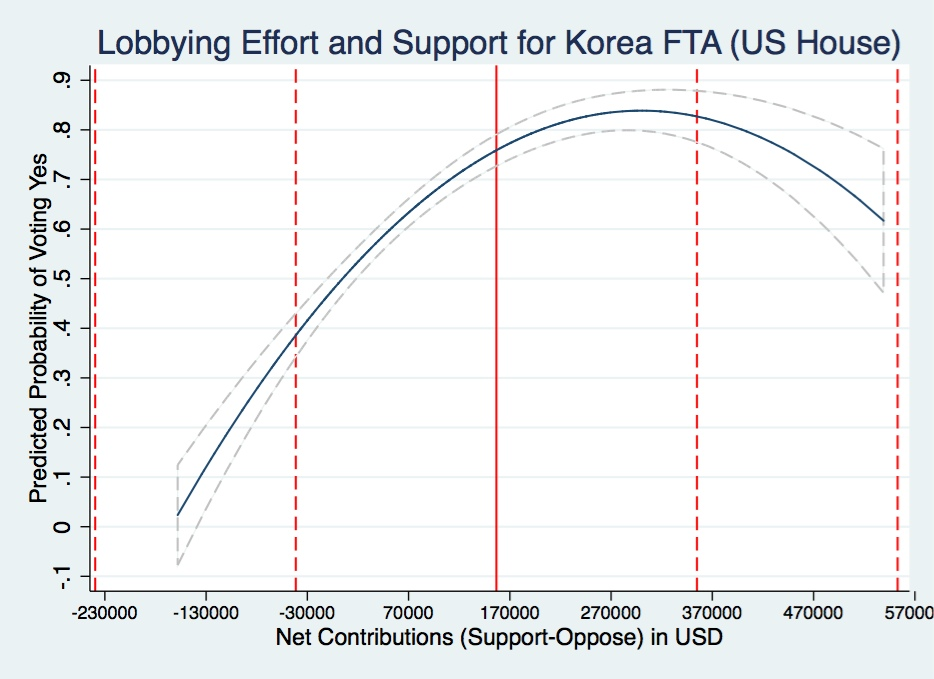
\includegraphics[width=2.9in]{graph2.jpg}
  \caption{Lobbying Effort and Support for KORUS
	\label{fig:br}}
\end{minipage}%
\begin{minipage}{.5\textwidth}
  \centering
  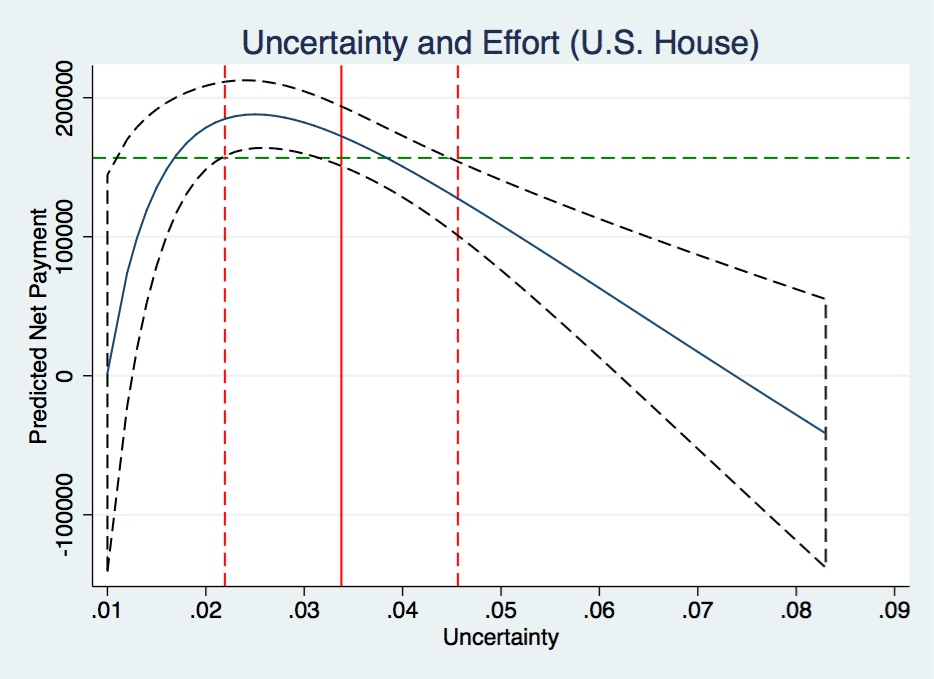
\includegraphics[width=2.9in]{graph1.jpg}
  \caption{Net Campaign Contributions, KORUS
	\label{fig:g1}}
\end{minipage}
\end{figure}

\textcolor{blue}{Figure 1 displays the relationship between lobbying effort and legislators' support for KORUS. The vertical axis represents the predicted probability that a legislator would vote ``yes'' on the agreement, and the horizontal axis shows the monetary contributions to each legislator by lobbies who supported the passage of KORUS minus the contributions from lobbies opposing the agreement. The solid vertical red line indicates the average net contribution in the sample, and the dashed lines a one-standard deviation increase/decrease from that sample mean. The data indicate that exporting industries are more likely to exert lobbying effort to enlist the support of additional legislators (extensive margin) rather than secure stronger support from a given set of legislators (intensive margin), as well as that there are decreasing returns to lobbying effort. To generate these results,  we regressed a legislator's vote on his/her estimated ideal point as well as partisanship using a probit specification. Then we fitted a second-order polynomial to the predicted probabilities generated by the probit regression. The contribution data for both this and the follow figure was obtained from Maplight.}

\textcolor{blue}{Figure 2 displays the relationship between the unpredictability of legislators' voting behavior and lobbying effort. The vertical axis represents the predicted net contributions to members of the U.S. House of Representatives in 2012, and the horizontal axis shows the unpredictability of legislator's voting behavior measured using the 95$\%$ posterior confidence intervals of their ideal points estimated using Bayesian Markov chain simulation to scale all roll call votes taken in the 112th Congress (more details on the methodology below). The solid vertical red line indicates the average uncertainty in the sample, and the vertical dashed red lines indicate increases/decreases of one-standard deviation from the average. The horizontal dashed green line indicates the predicted net payment in the sample. The data show a very strong relationship between uncertainty at the level of the individual legislator and campaign contributions. To generate these results, we fitted a second-order polynomial to the data, and used monetary contributions to each legislator by lobbies who supported the passage of KORUS minus the contributions from lobbies opposing the agreement. While these data do not map perfectly onto our theoretical constructs, they indicate that there is strong preliminary support for our hypotheses making it highly likely that investment in data acquisition and analysis is worthwhile.}



%\subsection{Break Decision}

%\subsection{Uncertainty for Select Interest Groups}
%\label{sec:select}


\section{Conclusion}
\label{sec:concl}



\section*{Appendix}

			




\newpage
\section*{References}

\begin{list}{}{\setlength{\leftmargin}{0.3in}\setlength{\rightmargin}{0.0in}\setlength{\itemindent}{-0.3in}\setlength{\itemsep}{0.0in}}


\item Ansolabehere, S., J. de Figueiredo, and J. Snyder Jr. (2003), ``Why Is There so Little Money in U.S. Politics?,'' {\em Journal of Economic Perspectives}, 17, 105-130.

\item Becker, G., (1983) ``A Theory of Competition among Interest Groups for Political Influence.'' {\em Quarterly Journal of Economics} 98, 371-400.

\item Bombardini, M. (2008), ``Firm Heterogeneity and Lobby Participation,'' {\em Journal of International Economics}, 75, 329-348.

\item Bombardini, M., and F. Trebbi (2012): ``Competition and Political Organization: Together or Alone in Lobbying for Trade Policy?'' {\em Journal of International Economics}, 87, 18-26.

\item Clinton, J., Jackman, S., and D. Rivers, (2004): ``The Statistical Analysis of Roll Call Data.'' {\em American Political Science Review}, 98, 355-370.

\item Dal Bo, E. (2007): ``Bribing Voters.'' {\em American Journal of Political Science} 51, 789-803.

\item Dekel, E., Jackson, M., Wolinsky, A. (2005): {\em Vote Buying.} Unpublished manuscript, Caltech.

\item Gawande, K., P. Krishna and M. Robbins (2006): ``Foreign Lobbies and U.S. Trade Policy,'' {\em Review of Economics and Statistics}, 88, 563-571.

\item Goldberg, P. and G. Maggi (1999): ``Protection for Sale: An Empirical Investigation,'' {\em American Economic Review}, 89, 1135-1155.

\item Groseclose, T., Snyder, J. M. (1996): ``Buying Supermajorities.'' {\em American Political Science Review} 90, 303-315.

\item Grossman, G. and E. Helpman (1994): ``Protection for Sale,'' {\em The American Economic Review}, 84, 833-850.

\item Grossman, G. and E. Helpman (2005): ``A Protectionist Bias in Majoritarian Politics,'' {\em The Quarterly Journal of Economics}, 120, 1239-1282.

\item Henisz, W. and E. Mansfield (2006), ``Votes and Vetoes: The Political Determinants of Commercial Openness,'' {\em International Studies Quarterly}, 50, 189-211.

\item Kibris, A. (2012), ``Uncertainty and Ratification Failure,'' {\em Public Choice}, 150, 439-467.

\item Laffont, J., Tirole, J. (1994): ``A Theory of Incentives in Procurement and Regulation.'' Cambridge: MIT Press.

\item Laver, M. and K. Shepsle (1991), ``Divided Government: America is Not `Exceptional','' {\em Governance: An International Journal of Policy and Administration}, 4, 250-269.

\item Le Breton, M. and F. Salanie (2003), ``Lobbying under political uncertainty,'' {\em Journal of Public Economics}, 87, 2589-2610.

\item Le Breton, M. and V. Zaporozhets (2007), ``Legislative Lobbying under Political Uncertainty,'' Available at SSRN: \url{http://ssrn.com/abstract=1024686}.

\item Peltzman, S. (1976), ``Toward a More General Theory of Regulation.'' {\em Journal of Law and Economics} 19, 211-248.

\item Poole, K. T. (2005), ``Spatial Models of Parliamentary Voting.'' New York: Cambridge University Press.

\item Saiegh, S. (2009), ``Political  Prowess or Lady Luck? Evaluating Chief Executives' Legislative Success Rates,'' {\em The Journal of Politics}, 71, 1342-1356.

\item Saiegh, S. (2011) ``Ruling by Statute: How Uncertainty and Vote-Buying Shape Lawmaking.'' New York: Cambridge University Press.

\item Stigler, G. (1975) ``The Citizen and the State: Essays on Regulation.'' Chicago: Chicago University Press.


\end{list}

\end{document}